If you haven't downloaded and unzipped \href{https://libaoj.in/courses/2021f/MATH3341/zip/Math.3341.zip}{\texttt{Math.3341.zip}}. Download and unzip it under \verb|H:| (H Drive if you are working on the Remote Lab). Change the current working directory by typing \verb|cd H:\Math.3341\Math.3341.Lab.07| in the Command Window, and type \verb|edit lab_07_script| in the Command Window to edit \verb|lab_07_script.m|.

%---------------------------------------------
\section{Debugging}
%---------------------------------------------
In this lab you will learn how to debug code and develop ways to make code more readable by employing good coding practices.

Your goal is to fix the bugs in \verb|lab_07_script.m| and \verb|lab_07_function.m|. These files solve the linear system $A \mathbf{x} = \mathbf{b}$ given by
\begin{align*}
    4 x_1 + 3 x_2       & = 24 \\
    3 x_1 + 4 x_2 - x_3 & = 30 \\
    - x_2 + 4 x_3       & = -24 \\
\end{align*}
using the Gauss-Seidel method with Successive Over Relaxation (SOR). This method gives means to speed up the convergence of our iterative method. The only change from the Gauss-Seidel method is the use of a parameter $\omega$. Depending on the choice of this $\omega$, the Gauss Seidel method can be performed in significantly less iterations than the original method. The iterative step in this method is now
$$
x_i^{(k)} = (1 - \omega) x_i^{(k-1)} + \frac{\omega}{a_{ii}} \left[ b_i - \sum_{j=1}^{i-1} a_{ij} x_j^{(k)} - \sum_{j=i+1}^{n} a_{ij} x_j^{(k - 1)} \right].
$$
These code files are riddled with various errors. Your task is to look through the code and correct all of the issues you encounter. Methods for doing this efficiently will be explained in the lab. Note that the necessary corrections may involve any of the following:

\begin{enumerate}[1.]
    \item changing variable names,
    \item fixing indexing,
    \item suppressing output,
    \item changing code style,
    \item adding proper indentation,
    \item adding comments,
    \item removing redundant code.
\end{enumerate}

Once you finish debugging, call \verb|diary('lab_07_output.txt')|, then run the script \verb|lab_07_script.m|, and call \verb|diary off| to save the output. The outputs and figures should be exactly same as those on the following pages. You will upload files \verb|sor_gauss_seidel.tex|, \verb|lab_07_script.m|, \verb|lab_07_function.m|, \verb|lab_07_output.txt|, \verb|lab_07_plot_1.pdf|, and \verb|lab_07_plot_2.pdf|. Recompile, and submit the generated \verb|.pdf| file on WyoCourses.

\newpage

\section{Results}

\subsection{Output}

\lstinputlisting[style=Plain]{../Math.3341.Lab.07.ans/lab_07_output.txt}

\subsection{Formatted output}

\begin{table}[!hbtp]
\caption{Solving the linear system using SOR}
\centering
\begin{tabular}{lrrrr}
\toprule
  iter &             $x$ &             $y$ &             $z$ &        residual \\
\midrule
$   0$ & $ 0.0000000000$ & $ 0.0000000000$ & $ 0.0000000000$ & $4.5292021f+01$ \\
$   1$ & $ 7.5000000000$ & $ 2.3437500000$ & $-6.7675781250$ & $1.6542021f+01$ \\
$   2$ & $ 3.4277343750$ & $ 3.4606933594$ & $-4.7266387939$ & $1.9972021f+00$ \\
$   3$ & $ 3.3986663818$ & $ 3.8465023041$ & $-5.1163083315$ & $1.3672021f+00$ \\
$   4$ & $ 3.0442374945$ & $ 3.9605554193$ & $-4.9832493486$ & $1.2852021f-01$ \\
$   5$ & $ 3.0259199208$ & $ 3.9907957980$ & $-5.0070639760$ & $9.1942021f-02$ \\
$   6$ & $ 3.0021489592$ & $ 3.9980789088$ & $-4.9988343470$ & $7.5592021f-03$ \\
$   7$ & $ 3.0012637832$ & $ 3.9996597426$ & $-5.0003977437$ & $5.0832021f-03$ \\
$   8$ & $ 3.0000030455$ & $ 3.9999579143$ & $-4.9999137159$ & $4.7242021f-04$ \\
$   9$ & $ 3.0000386940$ & $ 4.0000012096$ & $-5.0000211930$ & $2.2952021f-04$ \\
$  10$ & $ 2.9999891925$ & $ 4.0000032068$ & $-4.9999936996$ & $4.7792021f-05$ \\
$  11$ & $ 2.9999996955$ & $ 4.0000014526$ & $-5.0000011211$ & $9.0182021f-06$ \\
$  12$ & $ 2.9999987143$ & $ 4.0000004919$ & $-4.9999995660$ & $4.5162021f-06$ \\
$  13$ & $ 2.9999998603$ & $ 4.0000001436$ & $-5.0000000636$ & $4.7202021f-07$ \\
$  14$ & $ 2.9999999003$ & $ 4.0000000377$ & $-4.9999999723$ & $3.4342021f-07$ \\
$  15$ & $ 2.9999999896$ & $ 4.0000000090$ & $-5.0000000041$ & $3.0672021f-08$ \\
$  16$ & $ 2.9999999942$ & $ 4.0000000019$ & $-4.9999999984$ & $2.1392021f-08$ \\
$  17$ & $ 2.9999999996$ & $ 4.0000000004$ & $-5.0000000003$ & $1.7132021f-09$ \\
\bottomrule
\end{tabular}
\end{table}


\newpage

\subsection{Plots}
\begin{figure}[!hbtp]
    \centering
    \includegraphics[width=0.80\textwidth]{../Math.3341.Lab.07.ans/lab_07_plot_1.pdf}
    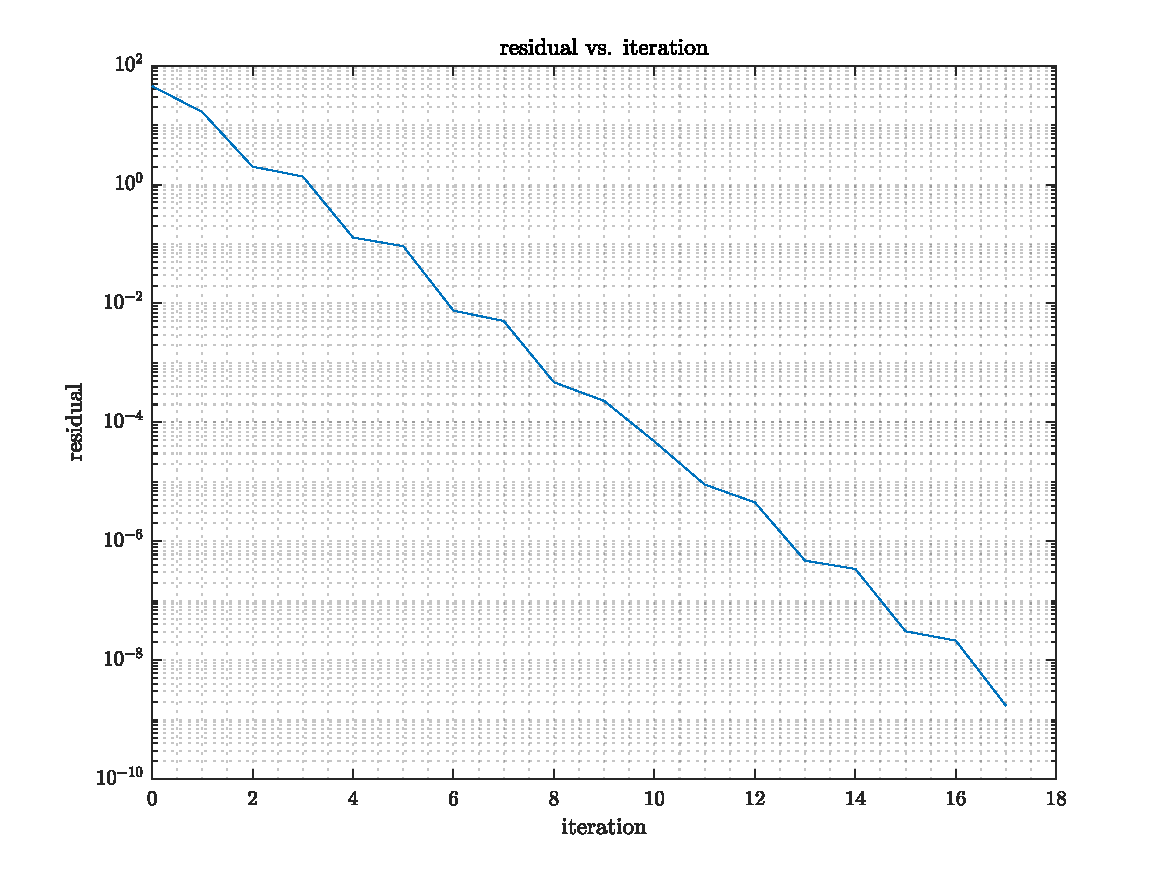
\includegraphics[width=0.80\textwidth]{../Math.3341.Lab.07.ans/lab_07_plot_2.pdf}
    \caption{Solution and residual}
    \label{fig:sol}
\end{figure}

